\documentclass[10pt,a4paper]{article}
\usepackage[UTF8,fontset = windows]{ctex}
\setCJKmainfont[BoldFont=黑体,ItalicFont=楷体]{华文中宋}
\usepackage{amssymb,amsmath,amsfonts,amsthm,mathrsfs,dsfont,graphicx}
\usepackage{ifthen,indentfirst,enumerate,color,titletoc}
\usepackage{tikz}
\usepackage{multicol}
\usepackage{makecell}
\usepackage{longtable}
\usepackage{diagbox}
\usetikzlibrary{arrows,calc,intersections,patterns,decorations.pathreplacing,3d,angles,quotes,positioning}
\usepackage[bf,small,indentafter,pagestyles]{titlesec}
\usepackage[top=1in, bottom=1in,left=0.8in,right=0.8in]{geometry}
\renewcommand{\baselinestretch}{1.65}
\newtheorem{defi}{定义~}
\newtheorem{eg}{例~}
\newtheorem{ex}{~}
\newtheorem{rem}{注~}
\newtheorem{thm}{定理~}
\newtheorem{coro}{推论~}
\newtheorem{axiom}{公理~}
\newtheorem{prop}{性质~}
\newcommand{\blank}[1]{\underline{\hbox to #1pt{}}}
\newcommand{\bracket}[1]{(\hbox to #1pt{})}
\newcommand{\onech}[4]{\par\begin{tabular}{p{.9\textwidth}}
A.~#1\\
B.~#2\\
C.~#3\\
D.~#4
\end{tabular}}
\newcommand{\twoch}[4]{\par\begin{tabular}{p{.46\textwidth}p{.46\textwidth}}
A.~#1& B.~#2\\
C.~#3& D.~#4
\end{tabular}}
\newcommand{\vartwoch}[4]{\par\begin{tabular}{p{.46\textwidth}p{.46\textwidth}}
(1)~#1& (2)~#2\\
(3)~#3& (4)~#4
\end{tabular}}
\newcommand{\fourch}[4]{\par\begin{tabular}{p{.23\textwidth}p{.23\textwidth}p{.23\textwidth}p{.23\textwidth}}
A.~#1 &B.~#2& C.~#3& D.~#4
\end{tabular}}
\newcommand{\varfourch}[4]{\par\begin{tabular}{p{.23\textwidth}p{.23\textwidth}p{.23\textwidth}p{.23\textwidth}}
(1)~#1 &(2)~#2& (3)~#3& (4)~#4
\end{tabular}}
\begin{document}

\begin{enumerate}[1.]
%gqj1
\item 对于集合$A=\{x|y=\dfrac{|x-1|}{x-1}, \ y\in \mathbf{R}\}$, $B=\{y|y=\dfrac{|x-1|}{x-1},\ x\in \mathbf{R},\ x\ne 1\}$, 下列说法中, 正确的说法的序号为\blank{50}.
\textcircled{1} $A\subset B$; \textcircled{2} $B\subset A$; \textcircled{3} $A\cap B\ne \varnothing$; \textcircled{4} $A\cap B=\varnothing$; \textcircled{5} $A\cap B=\mathbf{R}$.
\item 对于集合$C=\{(x,y)|y=x^2,\ x\in \mathbf{R}\}$, $D=\{(y,x)|y=x^2,\ x\in \mathbf{R}\}$, 则集合$C\cap D$的元素个数为\bracket{20}.
\fourch{$0$}{$1$}{$2$}{无限}
\item 设常数$m\in \mathbf{R}$. 已知集合$A=(2, 4)$, $B=(m, m^2)$. 若$A\subset B$, 求$m$的取值范围.
\item 设常数$a\in \mathbf{R}$. 已知集合$A=[2, 3]$, $B=[a, 2a-\dfrac 52]$, 且$A\cap B\ne \varnothing$, 求$a$的取值范围.
\item 设常数$a\in \mathbf{R}$.已知集合$A=\{x|x^2-(a+1)x+a=0\}$, $B=\{x|x^2-4x+2a=0\}$.\\
(1) 根据$a$的值, 写出集合$A$;\\
(2) 若$B\subseteq A$, 求$a$的值的集合.
\item 设常数$a\in \mathbf{R}$. 若$\{x|x^2-ax+a=0,\ x\in \mathbf{R}\}\cap  (-\infty , 0]\ne \varnothing$, 则$a$的取值范围为为\blank{50}.
\item 集合$A=\{(x,y)|x^2+y^2=25\}$, $B=\{(x,y)|(x-3)^2+(y-4)^2=100\}$, 则集合$A\cap B$的元素个数为\bracket{20}.
\fourch{$0$}{$1$}{$2$}{无限}
\item 设常数$a\in \mathbf{R}$. 已知集合$A=\{x|y=\sqrt {-1-\dfrac 1{1+x}}$且$x\in \mathbf{R}\}$, $B=\{x| ax<x+1, \ x\in \mathbf{R}\}$. 若$A\cap B=A$, 求$a$的取值范围.
\item 设常数$a\in \mathbf{R}$. 若关于$x$的不等式组$\begin{cases} x^2+2x-3\ge 0, \\  (x-2)(x-a)<0 \\ \end{cases}$整数解的集合为$\{1\}$, 则$a$的取值范围为\blank{50}.
\item 设常数$a\in \mathbf{R}$. 若$A=\{(x,y)|y=-x^2+ax, \ x\in \mathbf{R}\}$, $B=\{(x,y)|x+y=2,\ x\in [0,2]\}$. 记$A\cap B$的子集的个数为$n$.\\
(1) $n=2$, 求$a$的取值范围;\\
(2) 求$a$的取值范围, 使得$n$最大, 并求出对应的$n$的最大值.
\item 对于实数$x,y$, ``$x+y<4$''是``$x,y$中至少有一个小于等于$2$''成立的\bracket{20}条件.
\fourch{充分而不必要}{必要而不充分}{充分必要}{既不充分也不必要}
\item 对于$x,y\in \mathbf{R}$, 命题``$x+y\ne 4$''是命题``$x\ne 1$或$y\ne 3$''成立的\bracket{20}条件.
\fourch{充分而不必要}{必要而不充分}{充分必要}{既不充分也不必要}
\item 设$a_1,b_1,c_1,a_2,b_2,c_2$均为非零实数, 不等式$a_1x^2+b_1x+c_1>0$和$a_2x^2+b_2x+c_2>0$的解集分别为集合$M$和$N$, 那么``$\dfrac{a_1}{a_2}=\dfrac{b_1}{b_2}=\dfrac{c_1}{c_2}$''是``$M=N$''的\bracket{20}条件.
\fourch{充分而不必要}{必要而不充分}{充分必要}{既不充分也不必要}
\item 下列函数中, 最小值为$2$的函数的序号是\blank{50}.\\
\textcircled{1} $y=\cos x+\sec x$, $x\in (-\dfrac{\pi}2, \dfrac{\pi}2)$; \textcircled{2} $y=\cos x+\sec x$, $x\in (0,\dfrac{\pi}{2})$; \textcircled{3} $y=\ln x^2+\log_{x^2}\mathrm{e}$; \textcircled{4} $y=2^x+2^{-x}$, $x>0$; \textcircled{5} $y=\dfrac x{\sqrt {x-1}}$.
\item 设$a>0$, $a\ne 1$, $t>0$, 比较$a^{2t}$和 $a^{t^2-3}$的大小, 并证明你的结论.
\item 已知$x,y\in \mathbf{R}^+$, $x-y=1+xy$, 求$x-4y$的取值范围.
\item 设常数$a\in (0, 1)$.若$0<x\le y$, $a^x+a^y=1$. 已知$x+y$恰存在最小值与最大值中的一个, 请你指出$x+y$存在的是哪一个最值? 并求出该最值.
\item 设常数$a, b\in \mathbf{R}$, 关于$x$的不等式$(a^2-3b^2)x-ab<0$的解集是$(\dfrac 12, +\infty)$, 则$\dfrac ba=$\blank{50}.
\item 设常数$a\in \mathbf{R}$. 知函数$f(x)=x^2-2ax+4$. 若对任意$x\in [-1, 2]$, $f(x)>0$恒成立, 则$a$的取值范围为\blank{50}.
\item 设实数$m, n, p, q$满足不等式组$\begin{cases} (p-m)(p-n)>0, \\  (q-m)(q-n)<0, \\ (p-m)(q-m)>0, \\  m+n>p+q, \end{cases}$则$m, n, p, q$的大小顺序用``$<$''连接为\blank{50}.
\item 不等式$\ln x^2<\ln (4-3x)$的解集是\blank{50}.
\item 不等式$\log_2(1-x)>1+\log_4x$的解集是\blank{50}.
\item 设常数$a>0$. 已知关于$x$的不等式$(x-a)(x-2a)<0$的解集为$A$. 若$A\cap \mathbf{Z}$的元素个数为$3$, 求$a$的取值范围.
\item 不等式$\dfrac{3|x|-2}{|x|}\le 1$的解集是\blank{50}.
\item 设常数$a>0$且$a\ne 1$. 若关于$x$的不等式$\log_ax<0$的解集是$(1,+\infty)$, 则关于$x$的不等式$\log_a(x-\dfrac 4x)\ge 0$的解集是\blank{50}.
\item 设常数$a\in \mathbf{R}$. 已知关于$x$的不等式$\dfrac{ax-2}{x^2-a}<0$的解集为$M$. 若$1\in M$且$3\notin M$, 求$a$的取值范围.
\item 设$a,b,c$是互不相等的正数, 则下列不等式中正确的不等式的序号是\blank{50}.\\
\textcircled{1} $|a-c|\le |a-b|+|c-b|$; \textcircled{2} $a+\dfrac 1a\le a^3+\dfrac 1{a^3}$; \textcircled{3} $a-\dfrac 1a\le (a+b)^2-\dfrac 1{(a+b)^2}$; \textcircled{4} $\sqrt {a+4}+\sqrt {a+1}\le \sqrt {a+3}+\sqrt {a+2}$; \textcircled{5} $\sqrt {a+b+c}<\sqrt {abc}$.

%gqj2
\item 函数$y=f(x)$满足对于任意$x\ne 0$, 恒有$f(x-\dfrac 1x)=x^2+\dfrac 1{x^2}$. 若存在$x_0$使得$f(x_0)-x_0=2$成立, 则$x_0=$\blank{50}.
\item 已知半径为$r$的扇形的面积为$1$, 试将扇形的周长$C$表示成$r$的函数.
\item 设常数$a>1$. 已知函数$f(x)=\log_{\frac 12}(x^2-ax+2)$($1<x<a$). 若函数$y=f(x)$存在最大值, 求$a$的取值范围, 并求出对应的最大值.
\item 已知$xy<0$, 且$x^2-4y^2=4$. 问: 能否由此条件将$y$表示成$x$的函数? 若能, 求出该函数的解析式、定义域; 若不能, 说明理由.
\item 判断函数$f(x)=\begin{cases} \dfrac x{1-x}, &x\ge 0, \\ \dfrac x{1+x}, & x<0  \end{cases}$的奇偶性.
\item 根据常数$a$的不同取值, 讨论函数$f(x)=\dfrac{2^x+a}{2^x-a}$的奇偶性, 并说明理由.
\item 设常数$a\in \mathbf{R}$. 已知函数$y=f(x)$是定义在$\mathbf{R}$上的奇函数, 当$x<0$时, $f(x)=x+\dfrac{a^2}x$, 则$x\ge 0$时, $f(x)=$\blank{50}.
\item 设函数$y=f(x)$是定义在$\mathbf{R}$上的奇函数, 当$x>0$时, $f(x)=2^{\frac 1x}-3$. 求不等式$f(x)>-1$的解集.
\item 设函数$y=f(x)$为$\mathbf{R}$上的奇函数, 且对于任意$x\in \mathbf{R}$, 都有$f(x)=f(2-x)$. 当$1\le x<2$时, $f(x)=-2x+4$.\\
(1) 求函数$y=f(x)$在$-1\le x<1$时的解析式;\\
(2) 求函数$y=f(x)-1$在$-100\le x\le 100$时的所有零点的个数.
\item 已知定义在$\mathbf{R}$上的函数$y=f(x)$是奇函数, 且$y=f(x)$也是以2为周期的一个周期函数.若$f(\dfrac 32)=0$, 则在区间$[-2,2]$上的零点的个数的最小值为\blank{50}.
\item 函数$y=\dfrac 1{\sqrt {x^2-5x-6}}$的递增区间是\blank{50}.
\item 设常数$a\in \mathbf{R}$. 已知函数$y=f(x)$为$\mathbf{R}$上的奇函数, 且满足对于$(-\infty , +\infty)$内的任意$x_1$、$x_2$, 当$x_1<x_2$时, 都有$f(x_1)<f(x_2)$. 若$x>0$时, $f(x)=(x-a)^2-1$, 则$a$的取值范围为\blank{50}.
\item 判断函数$f(x)=2^x+2^{-x}$在$[0,+\infty)$上的单调性, 并证明你的结论.
\item 函数$f(x)=\ln (ax^2-4x+3)$在$(-\infty , 1]$上为减函数, 求实常数$a$的取值范围.
\item 下列命题中, 正确的命题的序号是\blank{50}.\\
\textcircled{1} 一个幂函数或是奇函数, 或是偶函数;\\
\textcircled{2} 当$\alpha =0$时, 函数$y=x^{\alpha }$的图像是一条射线;\\
\textcircled{3} 当$\alpha <0$且$y=x^{\alpha }$是奇函数时, 它的图像总是过$(-1,-1)$;\\
\textcircled{4} 若一个幂函数的图像经过第二象限的点, 则这个幂函数是偶函数.
\item 若集合$A=\{y|y=x^3, \ -1\le x\le 1\}$, $B=\{y|y=x^{-1}\}$, 则$A\cap B$等于\bracket{20}.
\fourch{$\{(-1,1)\}$}{$\{(1,1),(-1,-1)\}$}{$\{-1,1\}$}{$[-1,0)\cup (0,1]$}
\item 设常数$n\in \mathbf{Z}$. 若$f(x)=x^{n^2+2n-3}$是偶函数, 且图像与两条坐标轴都无公共点, 则$n=$\blank{50}.
\item 若函数$f(x)=1-\sqrt {-x^2-2x}$($-2\le x\le -1$), 请在空白处画出函数$y=f^{-1}(x)$的大致图像.
\item 设常数$a,b\in \mathbf{R}$, $a\ne b$, 是否存在$a, b$使得函数$f(x)=\dfrac{ax+1}{bx+1}$存在反函数, 且反函数就是$y=f(x)$? 若存在, 求出$a, b$满足的条件; 若不存在, 说明理由.

%gqj3
\item 设集合$A=\{5, \log_2(a+3)\}$, $B=\{a,b\}$, 若$A\cap B=\{2\}$, 则$A\cup B=$\blank{50}.
\item 已知函数$f(x)=\log_3(\dfrac 4x+2)$, 则方程$f^{-1}(x)=4$的解为$x=$\blank{50}.
\item 方程$\sin 2x=\sin 3x$的解集是\blank{50}.
\item 函数$y=\ln (-x^2+2x+3)$的单调递减区间是\blank{50}.
\item 若函数$y=f(x)$的图像与$y=x+\dfrac 1x$的图像关于$x=1$轴对称, 则$f(x)=$\blank{50}.
\item 已知等差数列$\{a_n\}$中, $a_1=10$, 当且仅当$n=5$时, 前$n$项和$S_n$取得最大值, 则公差$d$的取值范围是\blank{50}.
\item 已知函数$f(x)=a\sin x+b\cos x$($x\in [a^2-2,a]$)是奇函数, 则$a+b=$\blank{50}.
\item 不等式$x^2-3>ax-a$对一切$3\le x\le 4$恒成立, 则符合要求的自然数$a$有\blank{50}个.
\item 在$\triangle ABC$中, 锐角$\angle B$所对的边$b=10$. $\triangle ABC$的面积$S_{\triangle ABC}=10$, 外接圆半径$R=13$, 则$\triangle ABC$的周长为\blank{50}.
\item 若函数$f(x)=|x-3|-\log_ax+1$无零点, 则$a$的取值范围为\blank{50}.
\item 已知$\log_ax=\log_by=-2$.若$a+b=2$, 则$x+y$的取值范围为\blank{50}.
\item 已知函数$f(x)$满足: \textcircled{1} 对任意$x\in (0, +\infty)$, 恒有$f(2x)=2f(x)$成立; \textcircled{2} 当$x\in (1,2]$时, $f(x)=2-x$. 若$f(a)=f(2015)$, 则满足条件的最小的正实数$a$是\blank{50}.
\item 已知函数$f(x)$定义域为$[a,b]$. 则``函数$f(x)$在$[a,b]$上为单调函数''是``函数$f(x)$在$[a,b]$上有最大值和最小值''的	\bracket{20}.
\twoch{充分但非必要条件}{必要但非充分条件}{充要条件}{既非充分也非必要条件}
\item 若$\dfrac 1a<\dfrac 1b<0$, 有下面四个不等式: \textcircled{1} $|a|>|b|$; \textcircled{2} $a<b$; \textcircled{3} $a+b<ab$; \textcircled{4} $a^3>b^3$. 其中, 不正确的不等式有\bracket{20}.
\fourch{$0$个}{$1$个}{$2$个}{$3$个}
\item 已知: 数列$\{a_n\}$满足$a_1=16$, $a_{n+1}-a_n=2n$. 则$\{\dfrac{a_n}n\}$的最小值为\bracket{20}.
\fourch{$8$}{$7$}{$6$}{$5$}
\item 设函数$f_1(x)=\log_4x-(\dfrac 14)^x$、$f_2(x)=\log_{\frac 14}x-(\dfrac 14)^x$的零点分别为$x_1$与$x_2$, 则\bracket{20}.
\fourch{$0<x_1x_2<1$}{$x_1x_2=1$}{$1<x_1x_2<2$}{$x_1x_2\ge 2$}
\item 关于$x$的不等式$\dfrac{x-a}{x+1}>0$的解集$P$, 不等式$\log_2(x^2-1)\le 1$的解集为$Q$. 若$Q\subseteq P$, 求实数$a$的取值范围.
\item 已知: 函数$f(x)=p\sin \omega x\cdot \cos \omega x-\cos ^2\omega x$($p>0$, $\omega >0$)的最大值为$\dfrac 12$, 最小正周期为$\dfrac{\pi}2$.\\
(1) 求: $p$, $\omega$的值与$f(x)$的解析式;\\
(2) 若$\triangle ABC$的三条边为$a$, $b$, $c$, 满足$a^2=bc$, $a$边所对的角为$A$. 求: 角$A$的取值范围及函数$f(A)$的值域.
\item 市场上有一种新型的强力洗衣液, 特点是去污速度快. 已知每投放$a$($1\le a\le 4$, 且$a\in \mathbf{R}$)个单位的洗衣液在一定量水的洗衣机中, 它在水中释放的浓度$y$(克/升)随着时间$x$(分钟)变化的函数关系式近似为$y=a\cdot f(x)$, 其中$f(x)=\begin{cases} \dfrac{16}{8-x}-1, & 0\le x\le 4 \\ 5-\dfrac 12x, & 4<x\le 10. \end{cases}$ 若多次投放, 则某一时刻水中的洗衣液浓度为每次投放的洗衣液在相应时刻所释放的浓度之和. 根据经验, 当水中洗衣液的浓度不低于$4$(克/升)时, 它才能起到有效去污的作用.\\
(1) 若只投放一次$4$个单位的洗衣液, 则有效去污时间可达几分钟?\\
(2) 若第一次投放$2$个单位的洗衣液, $6$分钟后再投放$a$个单位的洗衣液, 要使接下来的$4$分钟中能够持续有效去污, 试求$a$的最小值(按四舍五入精确到$0.1$)
\item 设等差数列$\{a_n\}$的前$n$项和为$S_n$, 已知$a_2=4$, $S_5=30$.\\
(1) 求$a_n$的表达式;\\
(2) 设$A_n$为数列$\{\dfrac{a_n-1}{a_n}\}$的前$n$项积, 是否存在实数$a$, 使得不等式$A_n\cdot \sqrt {2n+1}<a$对一切$n\in \mathbf{N}^*$都成立? 若存在, 求出$a$的取值范围; 若不存在, 请说明理由;\\
(3) 将数列$\{a_n\}$依次按$1$项, $2$项, $3$项, $1$项, $2$项, $3$项循环地分为$(a_1)$, $(a_2,a_3)$, $(a_4,a_5,a_6)$, $(a_7)$, $(a_8,a_9)$, $(a_{10},a_{11},a_{12})$, $\cdots$, 分别计算各个括号内各数之和, 设由这些和按原来括号的前后顺序构成的数列为$\{b_n\}$, 求$b_{2015}$的值.
\item 已知函数$f_1(x)=\mathrm{e}^{|x-2a+1|}$, $f_2(x)=\mathrm{e}^{|x-a|+1}$($x\in \mathbf{R}$).\\
(1) 若$a=2$, 求$f(x)=f_1(x)+f_2(x)$在$x\in [2,3]$上的最小值;\\
(2) 若$|f_1(x)-f_2(x)|=f_2(x)-f_1(x)$对于任意的实数$x\in \mathbf{R}$恒成立, 求$a$的取值范围;\\
(3) 当$1\le a\le 6$时, 求函数$g(x)=\dfrac{f_1(x)+f_2(x)}2-\dfrac{|f_1(x)-f_2(x)|}2$在$x\in [1, 6]$上的最小值.


%gqj4

\item 方程$4^x-2^x=0$的解集为\blank{50}.
\item 若$(1-2\mathrm{i})\overline z=5+10\mathrm{i}$($\mathrm{i}$是虚数单位), 则$z=$\blank{50}.
\item 以$(1,2)$为圆心, 且与直线$4x+3y-35=0$相切的圆的方程是\blank{50}.
\item 无穷数列$\{a_n\}$, $a_n=(\dfrac 23)^n$, 则$\{a_n\}$的各项和为\blank{50}.
\item 等腰直角三角形的直角边长为$1$, 则绕斜边旋转一周所形成的几何体的体积为\blank{50}.
\item 若$(x-\dfrac ax)^9$的展开式中$x^3$的系数是$-84$, 则$a=$\blank{50}.
\item 抛物线$y^2=-12x$的准线与双曲线$\dfrac{x^2}9-\dfrac{y^2}3=1$的两条渐近线所围成的三角形的面积等于\blank{50}.
\item 设常数$\omega >0$, $t>0$, 函数$f(x)=\begin{vmatrix}
\sqrt 3 & \sin \omega x  \\ 1 & \cos \omega x  \end{vmatrix}$的最小正周期为$2\pi$, 将$f(x)$的图像向左平移$t$个单位, 所得图像对应的函数为偶函数, 则$t$的最小值为\blank{50}.
\item 两个三口之家, 共$4$个大人, $2$个小孩, 约定星期日乘红色、白色两辆轿车结伴郊游, 每辆车最多乘坐$4$人, 其中两个小孩不能独坐一辆车, 则不同的乘车方法种数是\blank{50}.
\item 向量$\overrightarrow  a$, $\overrightarrow  b$满足$|\overrightarrow  a|=1$, $|\overrightarrow  a-\overrightarrow  b|=\dfrac{\sqrt 3}2$, $\overrightarrow  a$与$\overrightarrow  b$的夹角为$60^\circ$, 则$|\overrightarrow  b|=$\blank{50}.
\item 数列$1,\dfrac 12,\dfrac 21,\dfrac 13,\dfrac 22,\dfrac 31,\dfrac 14,\dfrac 23,\dfrac 32,\dfrac 41,\cdots$, 则$\dfrac 89$是该数列的第\blank{50}项.
\item 已知直线$(1-a)x+(a+1)y-4(a+1)=0$(其中$a$为实数)过定点$P$, 点$Q$在函数$y=x+\dfrac 1x$的图像上, 则$PQ$连线的斜率的取值范围是\blank{50}.
\item 下列函数中, 是奇函数, 且在$(0,+\infty)$上递减的是\bracket{20}.
\fourch{$y=x^2$}{$y=x^3$}{$y=x^{-\frac 12}$}{$y=x^{-\frac 13}$}
\item 设$P$是$\triangle ABC$所在平面内一点. 若$\overrightarrow{CB}=\lambda \overrightarrow{PA}+\overrightarrow{PB}$, $\lambda \in \mathbf{R}$, 则点$P$一定在\bracket{20}.
\fourch{$\triangle ABC$内部}{$AC$边所在直线上}{$AB$边所在直线上}{$BC$边所在直线上}
\item 若$a,b$是异面直线, 则下列命题中的假命题为\bracket{20}.
\onech{过直线$a$可以作一个平面并且只可以作一个平面$\alpha$与直线$b$平行}{过直线$a$至多可以作一个平面$\alpha$与直线$b$垂直}{唯一存在一个平面$\alpha$与直线$a,b$等距}{可能存在平面$\alpha$与直线$a,b$都垂直}
\item 王先生购买了一部手机, 欲使用中国移动``神州行''卡或加入联通的$130$网, 经调查其收费标准见下表: (注: 本地电话费以分为计费单位, 长途话费以秒为计费单位)
\begin{center}
\begin{tabular}{|c|c|c|c|}
\hline
网络 & 月租费 & 本地话费 & 长途话费 \\ \hline
甲: 联通$130$ & $12$元 & $0.36$元/分 & $0.06$元/秒 \\ \hline
乙: 移动``神州行'' & 无 & $0.60$元/分 & $0.07$元/秒 \\ \hline
\end{tabular}
\end{center}
若王先生每月拨打本地电话的时间是拨打长途电话时间的$5$倍, 若要用联通$130$应最少打多长时间的长途电话才合算?  答: \bracket{20}.
\fourch{$300$秒}{$400$秒}{$500$秒}{$600$秒}
\item 在三棱锥$P-ABC$中, $PA$, $PB$, $PC$两两垂直, $PB=5$, $PC=6$. 若三棱锥$P-ABC$的体积为$20$, $Q$是$BC$的中点.
\begin{center}
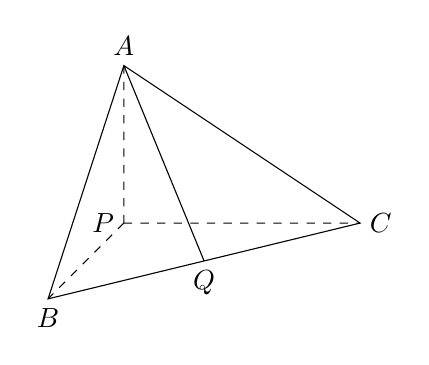
\begin{tikzpicture}[>=latex,scale = 0.5]
\draw (0,0,0) node [left] {$P$} coordinate (P);
\draw (6,0,0) node [right] {$C$} coordinate (C);
\draw (0,0,5) node [below] {$B$} coordinate (B);
\draw (0,4,0) node [above] {$A$} coordinate (A);
\draw ($(B)!0.5!(C)$) node [below] {$Q$} coordinate (Q);
\draw (A) -- (B) -- (C) -- cycle (A) -- (Q);
\draw [dashed] (P) -- (A) (P) -- (B) (P) -- (C);
\end{tikzpicture}
\end{center}
(1) 求$PA$;\\
(2) 求异面直线$PB$, $AQ$所成角的大小.
\item 已知角$ABC$是$\triangle ABC$的三个内角, $a,b,c$分别是角$A,B,C$的对边. 若向量$\overrightarrow m=(1-\cos(A+B),\cos\dfrac{A-B}2)$, $\overrightarrow n=(\dfrac 58,\cos\dfrac{A-B}2)$, 且$\overrightarrow  m\cdot \overrightarrow  n=\dfrac 98$.\\
(1) 求$\tan A\cdot \tan B$的值;\\
(2) 求$\dfrac{ab\sin C}{a^2+b^2-c^2}$的最大值.
\item 某市$2013$年发放汽车牌照$12$万张, 其中燃油型汽车牌照$10$万张, 电动型汽车$2$万张. 为了节能减排和控制总量, 从$2013$年开始, 每年电动型汽车牌照按$50\%$增长, 而燃油型汽车牌照每一年比上一年减少$0.5$万张, 同时规定一旦某年发放的牌照超过$15$万张, 以后每一年发放的电动车的牌照的数量维持在这一年的水平不变.
(1) 记$2013$年为第一年, 每年发放的燃油型汽车牌照数构成数列$\{a_n\}$, 每年发放的电动型汽车牌照数构成数列$\{b_n\}$, 完成下列表格, 并写出这两个数列的通项公式;
\begin{center}
\begin{tabular}{|c|c|c|c|c|}
\hline
$a_1=10$ & $a_2=9.5$ & $a_3=$\blank{30} & $a_4=$\blank{30} & $\cdots$ \\ \hline
$b_1=2$ & $b_2=3$ & $b_3=$\blank{30} & $b_4=$\blank{30} & $\cdots$ \\ \hline
\end{tabular}
\end{center}
(2) 从$2013$年算起, 累计各年发放的牌照数, 哪一年开始超过$200$万张?
\item 设常数$m\ne 0$. 已知椭圆$\dfrac{x^2}2+y^2=1$上两个不同的点$A,B$关于直线$y=mx+\dfrac 12$对称.
\begin{center}
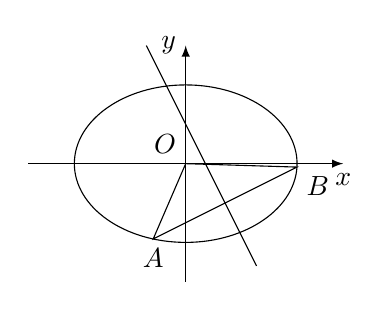
\begin{tikzpicture}[>=latex]
\draw [->] (-2,0) -- (2,0) node [below] {$x$};
\draw [->] (0,-1.5) -- (0,1.5) node [left] {$y$};
\draw (0,0) node [above left] {$O$};
\draw (0,0) ellipse ({sqrt(2)} and 1);
\draw [domain = -0.5:0.9] plot (\x, {-2*\x+1/2});
\draw ({1/2-sqrt(5/6)},{-1/2-sqrt(5/6)/2}) node [below] {$A$} coordinate (A) ({1/2+sqrt(5/6)},{-1/2+sqrt(5/6)/2}) node [below right] {$B$} coordinate (B);
\draw (0,0) -- (A) -- (B) -- cycle;
\end{tikzpicture}
\end{center}
(1) 若已知$C(0,\dfrac 12)$, $M$为椭圆上动点, 证明: $|MC|\le \dfrac{\sqrt {10}}2$;\\
(2) 求实数$m$的取值范围;\\
(3) 求$\triangle AOB$面积的最大值($O$为坐标原点).
\item 已知函数$f(x)=\log_k x$($k$为常数, $k>0$且$k\ne 1$), 且数列$\{f(a_n)\}$是首项为$4$, 公差为$2$的等差数列.\\
(1) 求证: 数列$\{a_n\}$是等比数列;\\
(2) 若$b_n=a_n+f(a_n)$, 当$k=\dfrac 1{\sqrt 2}$时, 求数列$\{b_n\}$的前$n$项和$S_n$的最小值;\\
(3) 若$c_n=a_n\lg a_n$, 问是否存在实数$k$, 使得$\{c_n\}$是递增数列? 若存在, 求出$k$的范围; 若不存在, 说明理由.


\end{enumerate}



\end{document}